%%%% 第一版 2020.10
%此文档为普通物理实验三林伟华老师要求的物理实验报告模板
%作者:武汉大学物理科学与技术学院18级詹睿知
%参考自电子信息学院实验报告模板
%%%% 第二版 2022.8
%更改优化了documentclass
\documentclass{WHUReport}
\usepackage{amsmath}
\usepackage{gbt7714}% 国标引用格式

%%%% 以下填写学生信息及实验题目
\newcommand{\major}{物理学}
\newcommand{\name}{郑卜凡}
\newcommand{\stuid}{2021302022016}
\newcommand{\Name}{Bufan Zheng}
\newcommand{\course}{普通物理实验三}
\newcommand{\newtitle}{利用保罗机械阱探求囚禁粒子的动力学特征}
\newcommand{\Title}{Study on the dynamics of trapped particles using the rotating-saddle trap}

\begin{document}
\pagestyle{maincontent} 
\bibliographystyle{plain}

\begin{center}
\zihao{-2} \textbf{\newtitle}\\
\zihao{7}~\\
\zihao{4} \kaishu \name \ \ (\stuid)\\
\zihao{5} \kaishu (武汉大学物理科学与技术学院,湖北省 武汉市 430072)\\
\end{center}
\zihao{-5}\textbf{摘\quad 要:}
%在此处修改中文摘要
在保罗机械阱上利用视频分析软件Tracker分析囚禁粒子的运动轨迹,形象地展现了囚禁粒子在势阱中的不同运动状态。控制不同变量重复进行多组实验,并将实验结果与Mathematica软件的理论分析进行了比较,解释了理论分析的不足所导致的与实验现象的差别。\\
\zihao{-5}\textbf{关键词:}Tracker;保罗机械阱;非线性动力学;Mathematica
~\\
\begin{center}
	\zihao{3}\textbf{\Title}\\
	\zihao{-4} \Name\quad (\stuid)\\
	\zihao{5} School of physical science and technology, Wuhan University, Wuhan, 430072, China
\end{center}

\zihao{5}\textbf{Abstract:}Using the motion video analysis software Tracker, the motion of particles in rotating-saddle trap was analyzed, and different motion states were shown. Multiple sets of experiments were repeated with different variables, and the experimental results were compared with the theoretical analysis of Mathematica software, which explained the difference between the experimental phenomenon caused by the lack of theoretical analysis.

\zihao{5}\textbf{Keywords: }Tracker; rotating-saddle trap; nonlinear dynamics; Mathematica

\begin{multicols}{2}
	离子阱是研究量子理论重要的实验装置。利用多级电势构成三维势阱,将离子稳定的囚禁在几乎与外界隔离的空间几何构型中的实验方法,称为离子囚禁技术\upcite{Has}。离子阱技术因其优良的特性和先进的功能,逐渐形成了一片新型广阔的研究领域,如量子信息\upcite{PhysRevA.62.042305}、量子逻辑门\upcite{PhysRevLett.74.4083}、离子阱频标\upcite{luo}、大规模光谱测量\upcite{PhysRevA.71.032504}等研究中具有广泛的应用。对于囚禁粒子动力学特性及其稳定条件是离子阱研究基础,但四级离子阱结构复杂,不宜直观地了解其中的各种运动过程及离子的稳定条件分析。保罗机械阱\upcite{paul}利用粒子在可旋转的对称马鞍面上的运动模拟粒子在势阱中的运动规律。本实验目的是探究保罗机械阱的稳定条件并在此基础上理解四级离子阱的工作机制。
	\section{实验原理}
	本节结合Mathematica软件数值计算来分析粒子在机械阱上的运动。
	\subsection{理论分析}
	如图1所示,在静止的马鞍面中我们取鞍点作为坐标原点建立直角坐标系,容易得到马鞍面中重力势场为
	\begin{equation}
		U(x_0,y_0)=\frac{mgh_0}{{r_0}^2}({x_0}^2{-y_0}^2)
	\end{equation}
	其中$h_0$为鞍点到马鞍面最高点的垂直距离,$r_0$为对称马鞍面的投影圆半径。现在考虑马鞍面以$\Omega$角速度开始旋转,在实验室参考系下重力势可表达为
	\begin{equation}
		U(x,y,t)=\frac{mgh_0}{{r_0}^2}\left[({x}^2{-y}^2)\cos(2\Omega t)+2xy\sin(2\Omega t)\right]
	\end{equation}
	考虑到粒子在马鞍面上垂直方向的速度相比于水平方向速度要小很多,所以$\dot{z}$可以忽略不计,另外不考虑摩擦力的作用,选取$x,y$为广义坐标可以写下拉格朗日量为
	\begin{equation}
		L=\frac{1}{2}m{\dot{x}}^2+\frac{1}{2}m{\dot{y}}^2-U(x,y,t)
	\end{equation}
	引入无量纲量
	\begin{equation}
		\tau\equiv \Omega t,\quad q\equiv\frac{gh_0}{{r_0}^2\Omega^2}
	\end{equation}
	由Euler-Lagrange方程可以得到粒子运动方程为
	\begin{align}
		\frac{d^2 x}{d \tau^2}+2q\left[x\cos(2 \tau)+y\sin(2\tau)\right]&=0\\
		\frac{d^2 y}{d\tau^2}-2q\left[y\cos(2 \tau)-x\sin(2\tau)\right]&=0
	\end{align}
	考虑在复平面上求解方程,定义$z=x+\mathrm{i}y$得到
	\begin{equation}
		\frac{d^2 z}{d\tau^2}+2q\bar {z}\mathrm{e}^{\mathrm{i}2\tau}=0
	\end{equation}
	不难发现方程的解具有形式
	\begin{equation}
		z(\tau)=f(\tau)\mathrm{e}^{\mathrm{i}\tau}
	\end{equation}
	其中
	\begin{equation}
		f(\tau)=A\mathrm{e}^{+\beta_+\tau}+B\mathrm{e}^{-\beta_+\tau}+C\mathrm{e}^{+\beta_-\tau}+D\mathrm{e}^{-\beta_-\tau}
	\end{equation}
	参数$\beta_\pm$满足
	\begin{equation}
		\beta_\pm=\sqrt{\pm 2|q|-1}
	\end{equation}
	
	从解的形式不难看出当且仅当$\beta_\pm$为纯虚数时,粒子在马鞍面中才能被囚禁,即稳定的平衡条件为
	\begin{equation}
		2q=\frac{2gh_0}{{r_0}^2\Omega^2}\le 1
	\end{equation}
	从上式可以看出粒子是否被囚禁与粒子的质量无关,马鞍面投影面积越大,鞍点到马鞍面最高点的垂直距离越小(对应马鞍面相对越平坦),马鞍面转速越大,粒子越容易被囚禁。
	\subsection{数值求解}
	原则上可以通过对初始条件分析得到四个待定系数$A,B,C,D$所满足的线性方程组从而对运动方程进行解析求解。这里考虑使用科学计算软件Mathematica直接对运动方程(5)(6)进行数值求解。
	
	在释放粒子时,都是在鞍点处释放,但是由于环境微扰,初始的速度不可能精确地等于0(否则从运动方程可以看出粒子将在鞍点处平衡),所以我们假设粒子有比较小的初速度$v_0=0.01\operatorname{cm/s}$。在不同的$q$下绘制运动图像。
	
	比较典型的图像是在$q$比较小时,这里取为$0.05$,绘制出一个周期以及多个周期的运动图像为:
	\begin{figure}[H]
		\centering
		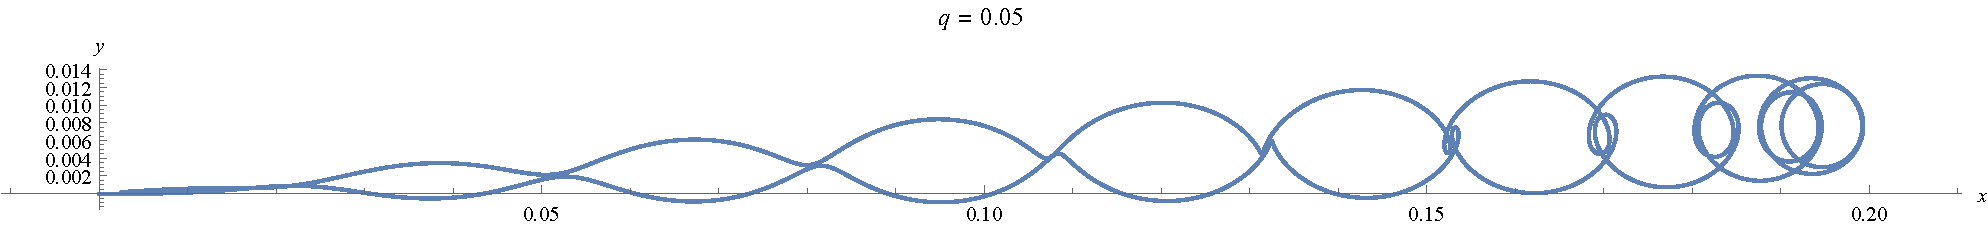
\includegraphics[width=\linewidth]{figures/0.05S.pdf}
		\caption{$q=0.05$时短周期下粒子运动图像}
	\end{figure}
	\begin{figure}[H]
		\centering
		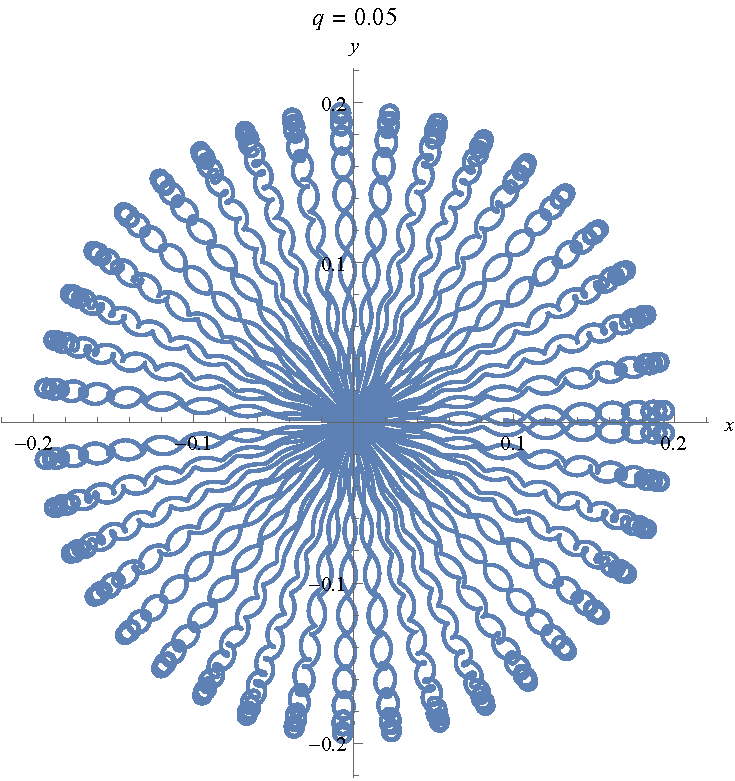
\includegraphics[width=0.5\linewidth]{figures/0.05L.pdf}
		\caption{$q=0.05$时长周期下粒子运动图像}
	\end{figure}
	其它$q<0.5$,即粒子被囚禁情况下运动图像为:
	\begin{figure}[H]
		\centering  %图片全局居中
		\subfigbottomskip=2pt %两行子图之间的行间距
		\subfigcapskip=-5pt %设置子图与子标题之间的距离
		\subfigure[$q$=0.1]{
			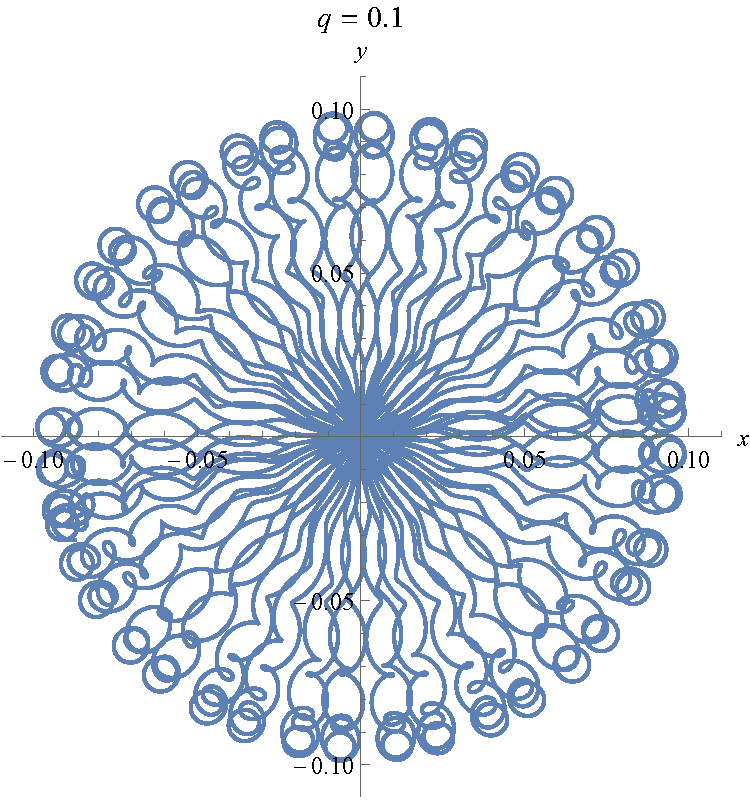
\includegraphics[width=0.48\linewidth]{./figures/0.1.pdf}}
		\subfigure[$q$=0.2]{
			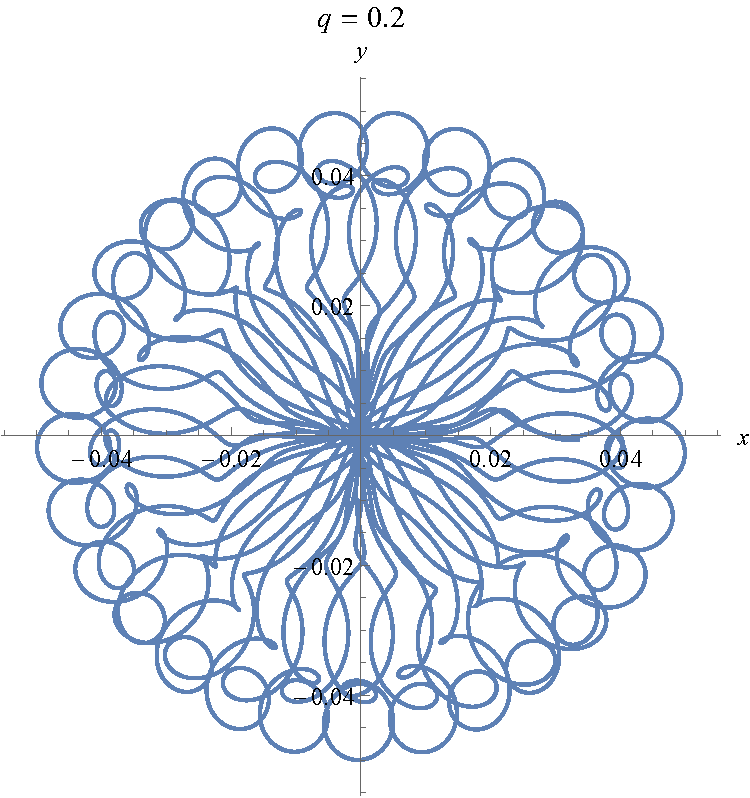
\includegraphics[width=0.48\linewidth]{./figures/0.2.pdf}}
		\\
		\subfigure[$q$=0.3]{
			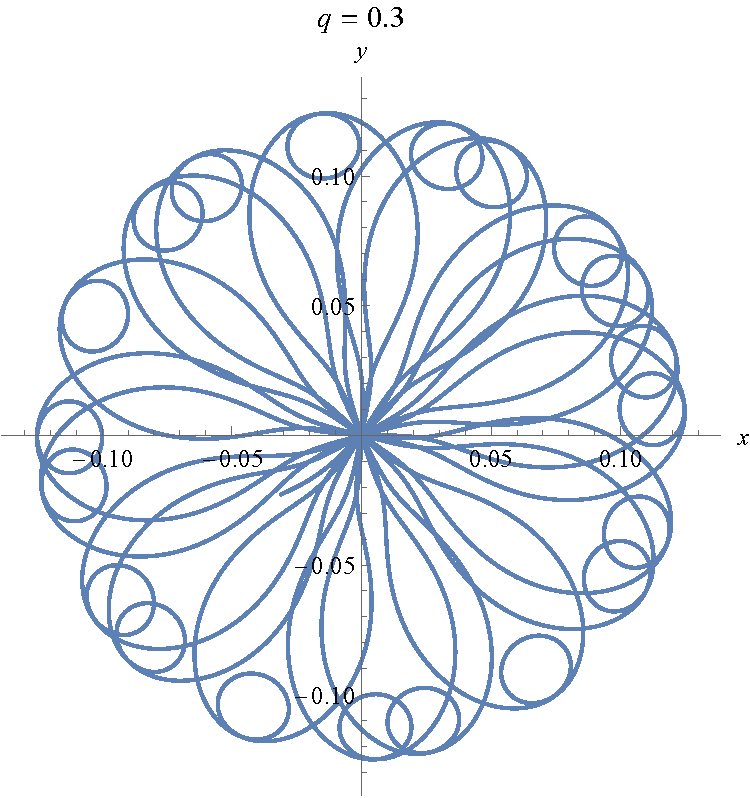
\includegraphics[width=0.48\linewidth]{./figures/0.3.pdf}}
		%\quad
		\subfigure[$q$=0.4]{
			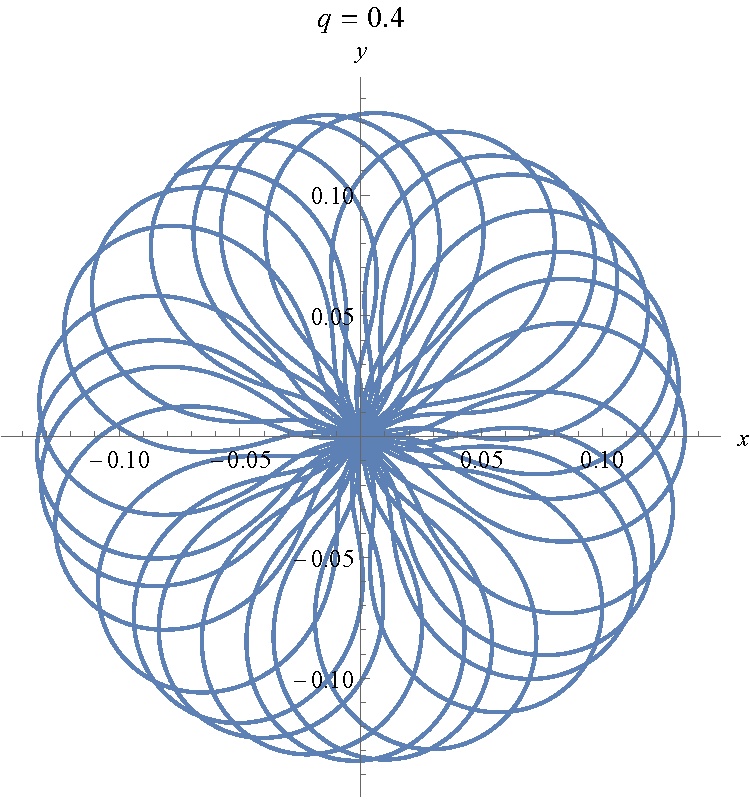
\includegraphics[width=0.48\linewidth]{./figures/0.4.pdf}}
		\caption{$q<0.5$时粒子的运动图像,有意思的是这些$q$值绘出来的图像都是规律性比较强的,但其它$q$值在长周期下规律性较差。}
	\end{figure}
	
	上图中可以很清晰地看出粒子运动图像随参数$q$的演化规律。而且可以看到明显的被囚禁现象。在临界值$q=0.5$附近粒子运动图像为:
	\begin{figure}[H]
		\centering  %图片全局居中
		\subfigbottomskip=2pt %两行子图之间的行间距
		\subfigcapskip=-5pt %设置子图与子标题之间的距离
		\subfigure[$q$=0.5]{
			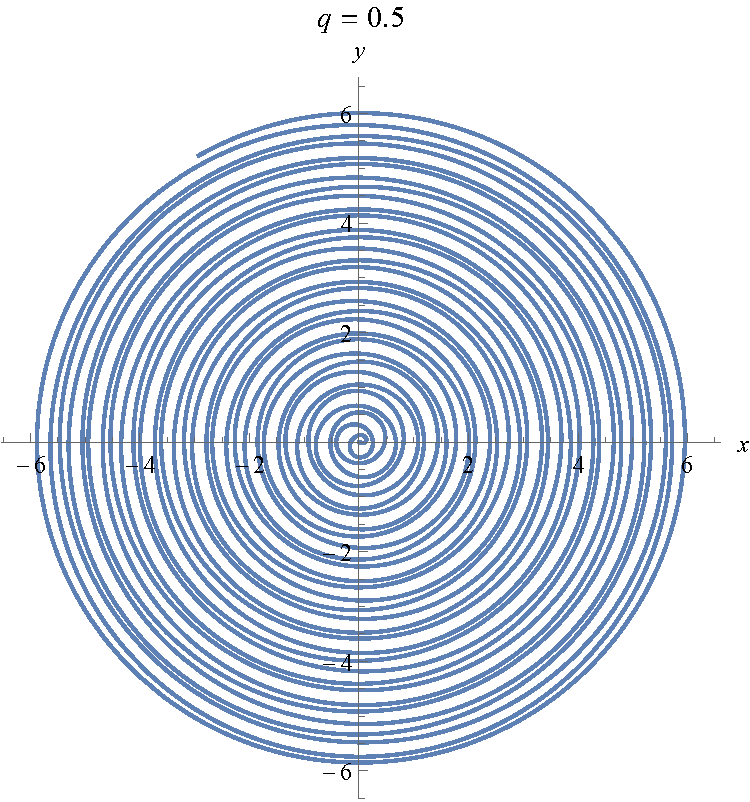
\includegraphics[width=0.48\linewidth]{./figures/0.5.pdf}}
		\subfigure[$q$=0.51]{
			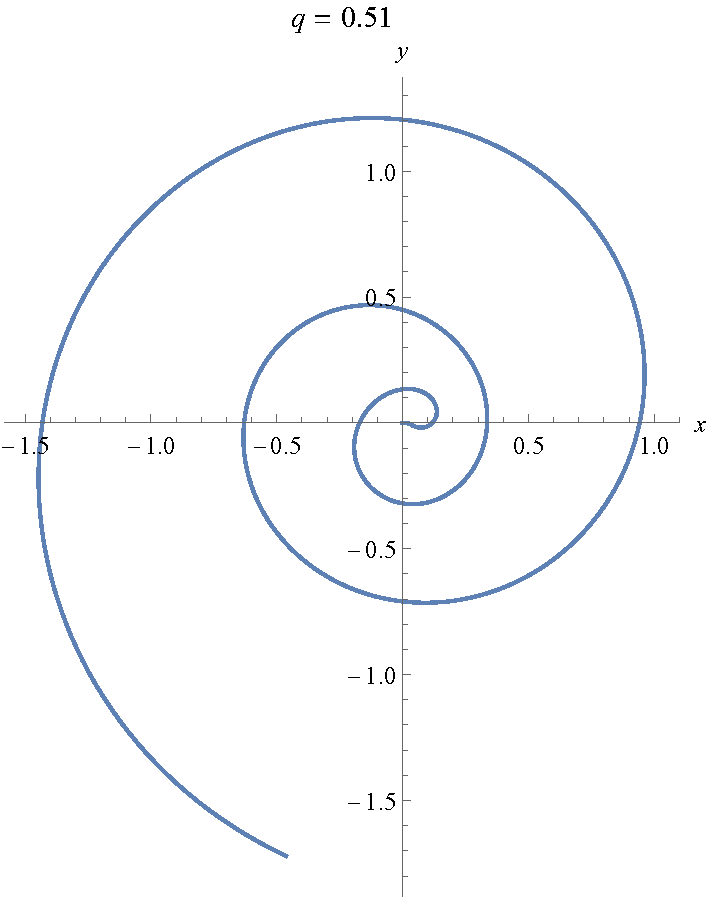
\includegraphics[width=0.48\linewidth]{./figures/0.51.pdf}}
		\caption{$q\sim0.5$时粒子的运动图像}
	\end{figure}
	
	可以直观地看到,在$q=0.5$时,粒子仍旧可以近似的认为被囚禁在小范围内运动,但一旦$q>0.5$,哪怕只有非常小的偏差,粒子的运动都会变成对数螺线,快速脱离马鞍面。
	
	\section{实验验证}
	实验装置如下图所示。利用卷尺测得马鞍面参数$r_0=17.45\operatorname{cm}$,$h_0=3.60\operatorname{cm}$,$g$取$9.8\operatorname{m/s^2}$。
	\begin{figure}[H]
		\centering
		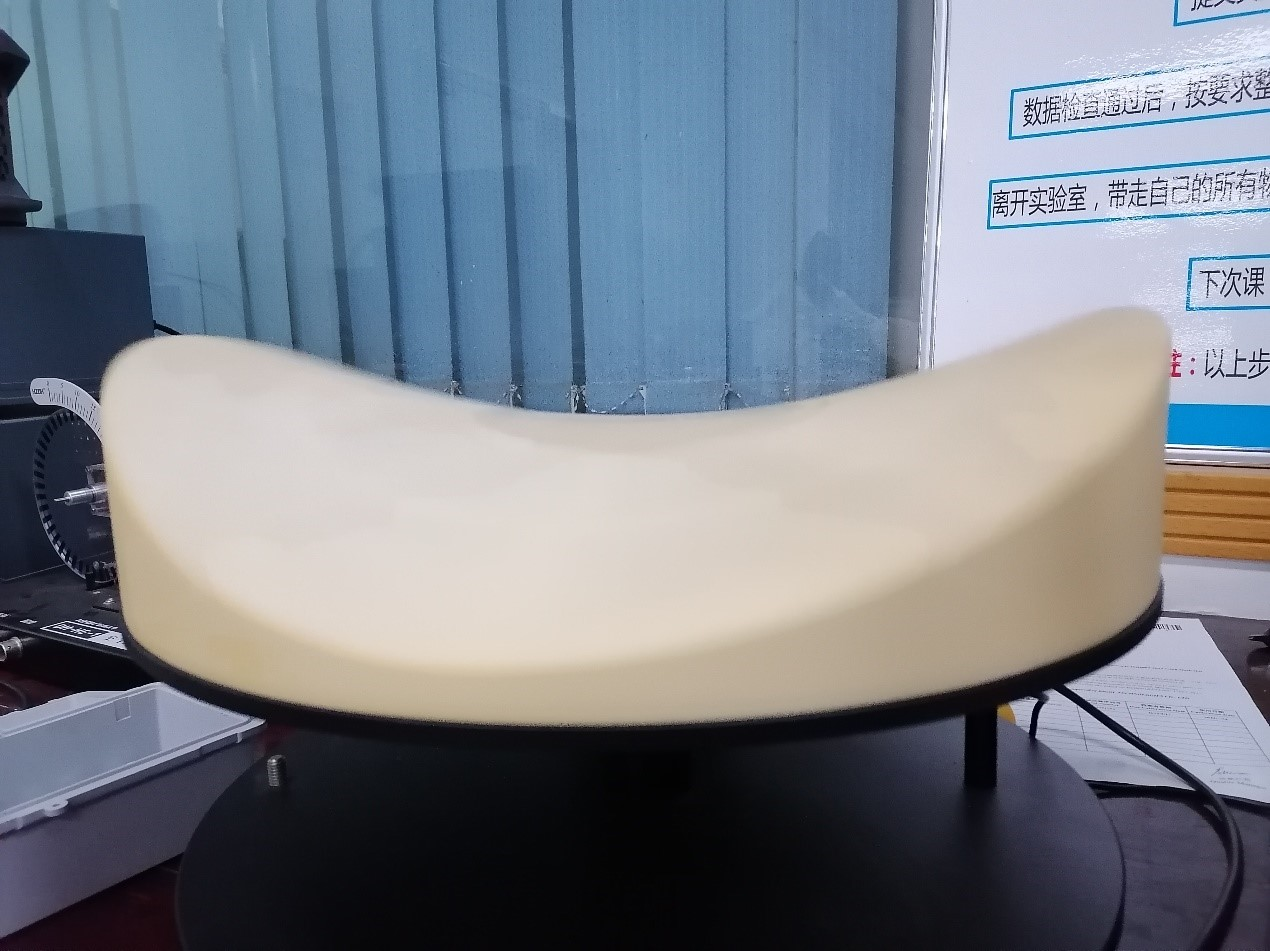
\includegraphics[width=0.4\textwidth]{figures/mechanic.jpg}
		\caption{实验装置侧面图}	
	\end{figure}
	\subsection{实验过程}
	实验室中的机械阱转速从$0\sim 200\operatorname{r/min}$可调,实验发现$ 40\operatorname{r/min}$转速以下,小球无法在势阱中被囚禁,会从鞍点直接滑落,所以实验从$ 40\operatorname{r/min}$到$ 200\operatorname{r/min}$每隔$ 20\operatorname{r/min}$进行一次实验。实验室中还有铝球、塑料小球和乒乓球三种不同大小不同质量的球作为“粒子”(下文分别以黑、白和橙球简称),实验中分别用三种小球进行实验,每组实验重复测量三次,待转速稳定后将小球垂直放入鞍点。然后录制视频并记录小球离开机械阱所用的时间。
	\subsection{实验数据处理}
	为了对拍摄到的图片更好地利用Tracker软件进行处理,首先利用AE软件对视频做防抖动处理,然后调节视频色彩对比度,突出小球,使得描点更加精确。
	\begin{figure}[H]
		\centering  %图片全局居中
		\subfigbottomskip=2pt %两行子图之间的行间距
		\subfigcapskip=-5pt %设置子图与子标题之间的距离
		\subfigure[处理前]{
			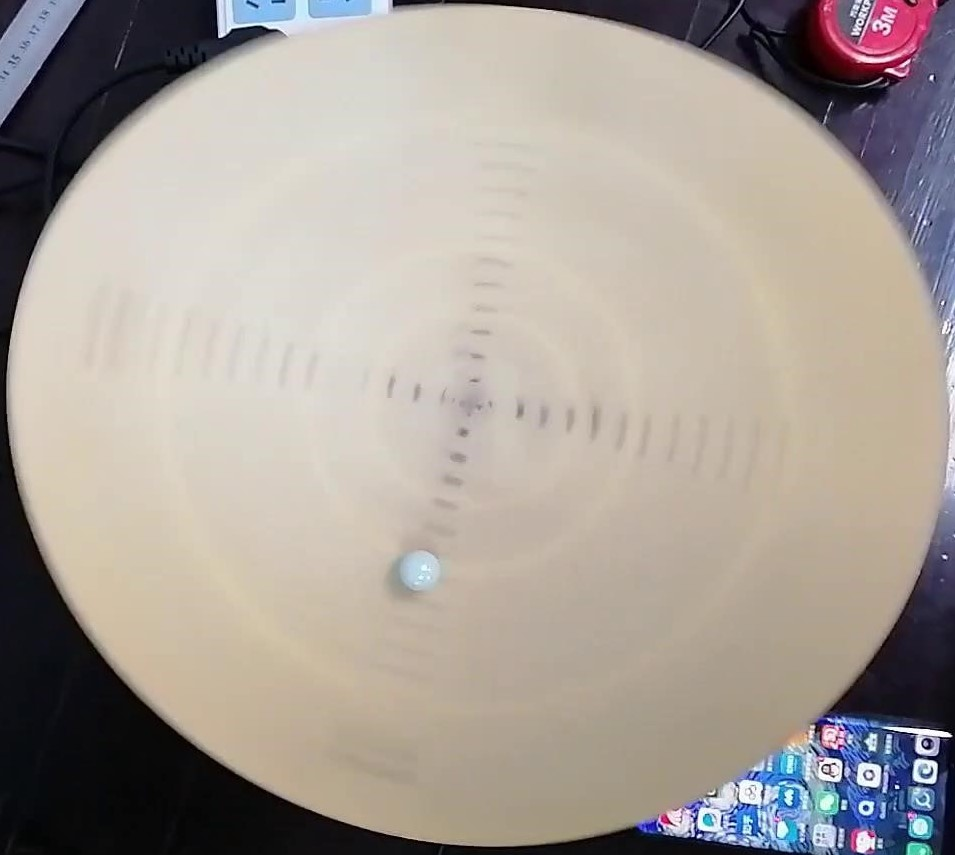
\includegraphics[width=0.48\linewidth]{./figures/before.jpg}}
		\subfigure[处理后]{
			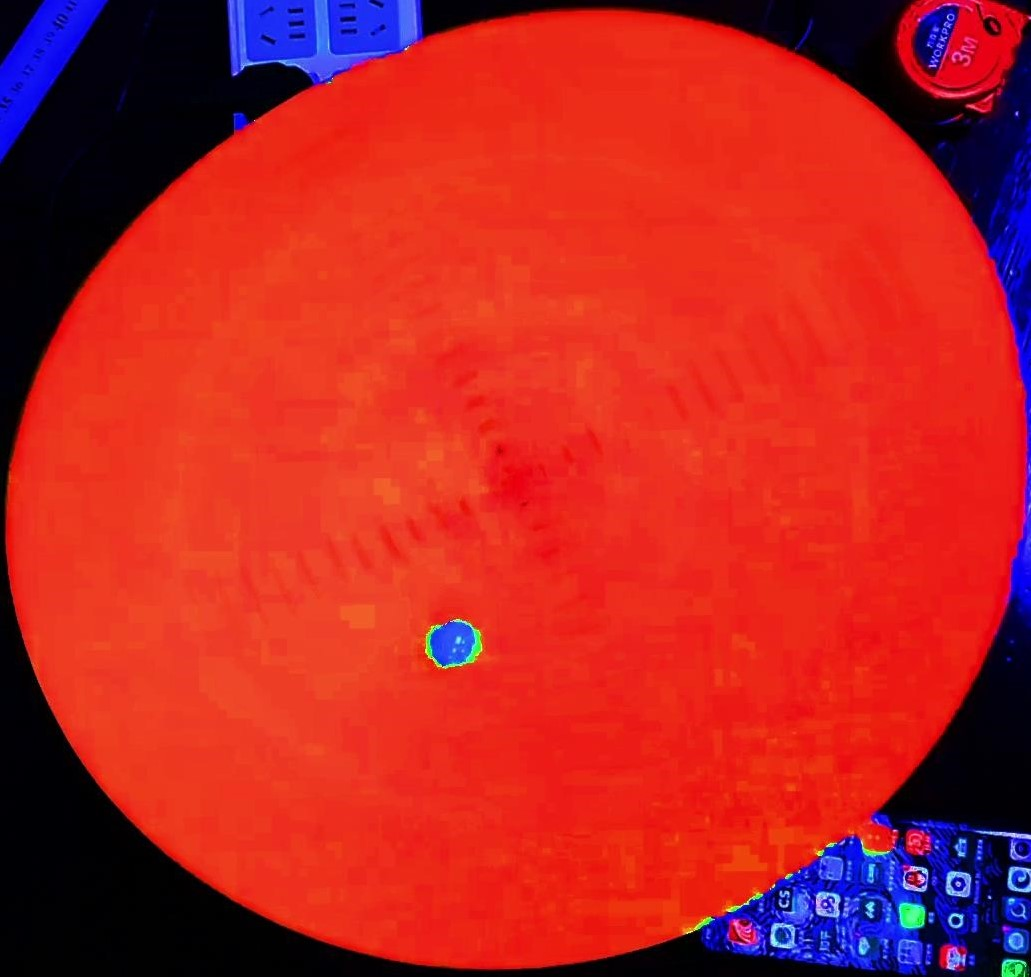
\includegraphics[width=0.48\linewidth]{./figures/after.jpg}}
		\caption{利用AE对视频进行初步处理,这里是对塑料小球视频的后期处理}
	\end{figure}
	
	利用Tracker进行分析,然后将数据导入MATLAB进行绘图得到运动轨迹。并带入数据计算相应的$q$值。
	\subsection{实验数据表达}
	首先是比较特殊的$40\operatorname{r/min}$,其$q$约为$0.6$,在临界值附近,其运动图像为:
	\begin{figure}[H]
		\centering  %图片全局居中
		\subfigbottomskip=2pt %两行子图之间的行间距
		\subfigcapskip=-5pt %设置子图与子标题之间的距离
		\subfigure[塑料小球]{
			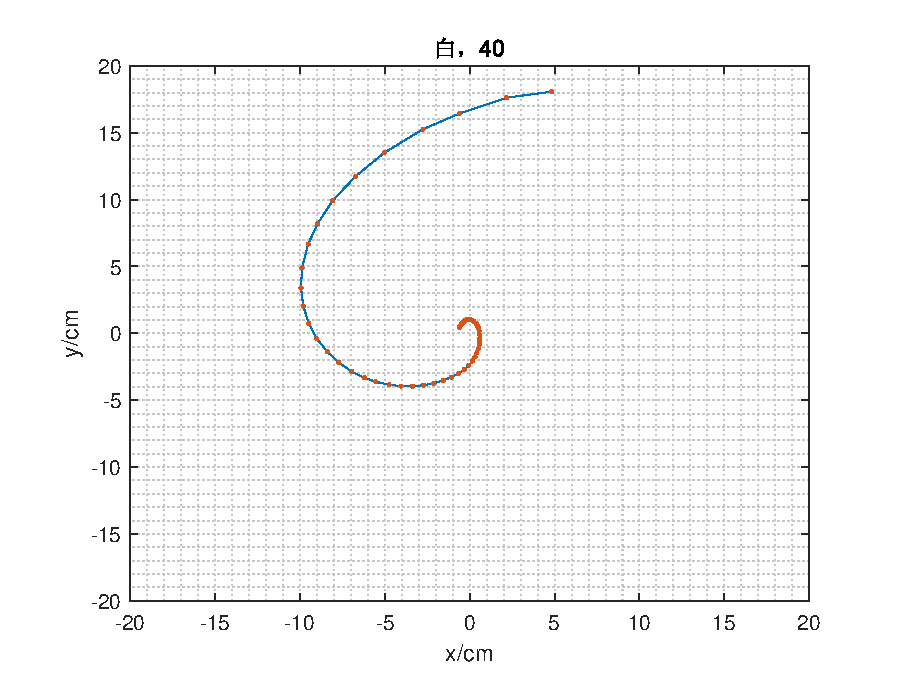
\includegraphics[width=0.48\linewidth]{./figures/w40.eps}}
		\subfigure[乒乓球]{
			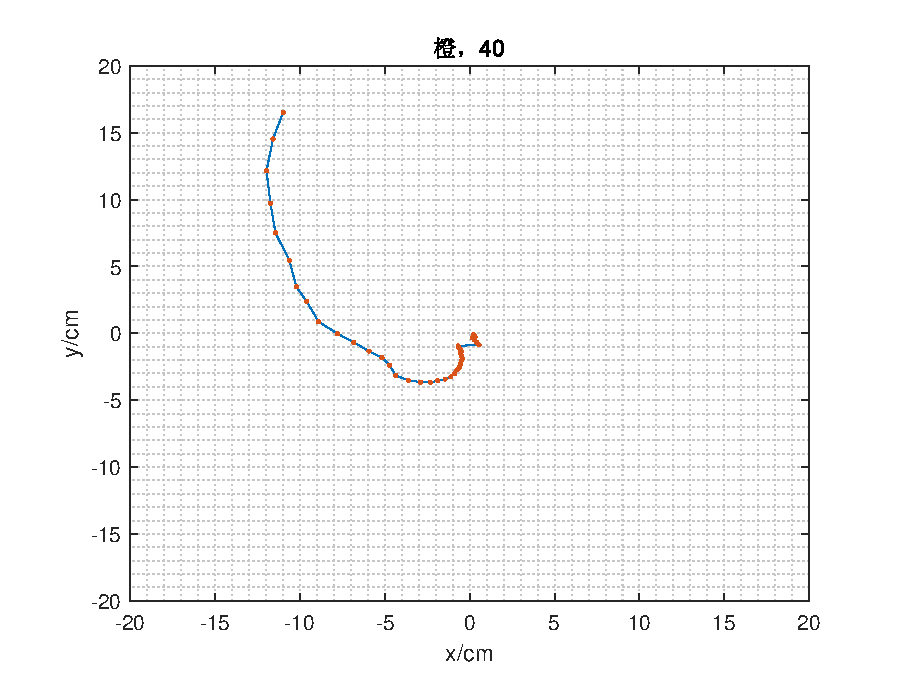
\includegraphics[width=0.48\linewidth]{./figures/o40.eps}}
		\caption{转速为$40\operatorname{r/min}$时的运动轨迹}
	\end{figure}
	
	这里可以明显地看到小球的运动轨迹为对数螺线,与图4-b相吻合。小于$40\operatorname{r/min}$的其它转速下小球的运动轨迹也是类似的对数螺线,我们比较感兴趣的是$q\geq0.5$的情况下小球的运动轨迹。
	\subsubsection{塑料小球}
	\begin{figure}[H]
		\centering  %图片全局居中
		\subfigbottomskip=2pt %两行子图之间的行间距
		\subfigcapskip=-5pt %设置子图与子标题之间的距离
		\subfigure[$q$=0.318]{
			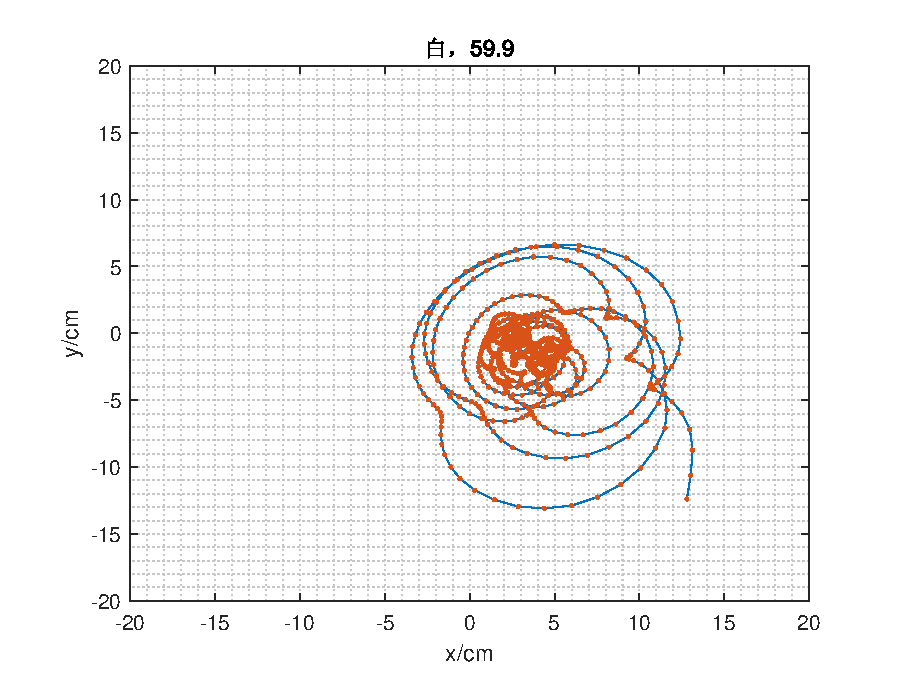
\includegraphics[width=0.48\linewidth]{./figures/w60.eps}}
		\subfigure[$q$=0.179]{
			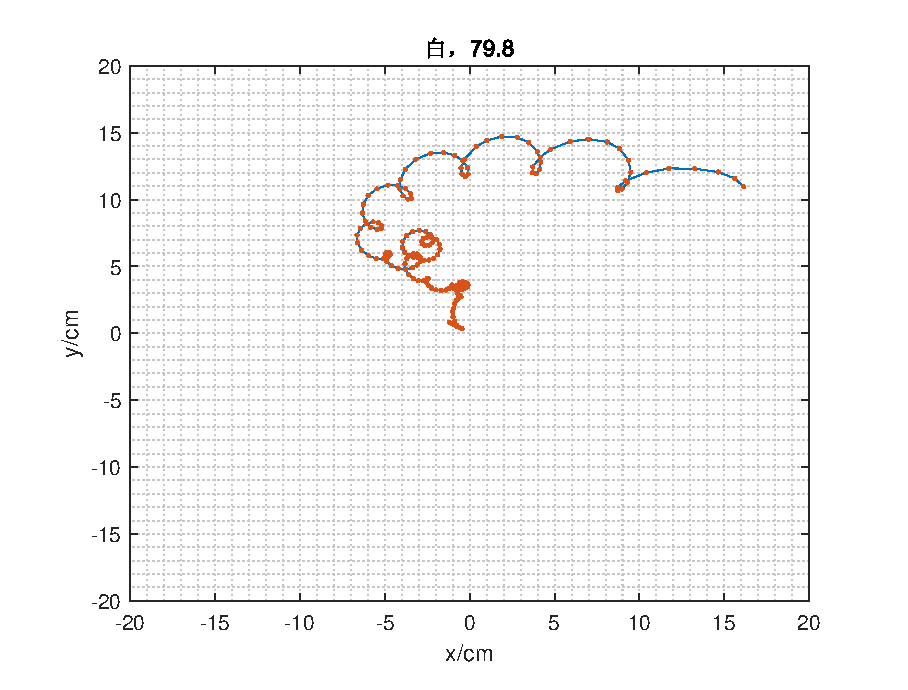
\includegraphics[width=0.48\linewidth]{./figures/w80.eps}}
	\end{figure}
	\addtocounter{figure}{-1} 
	\begin{figure}[H]
		\addtocounter{figure}{1} 
		\centering  %图片全局居中
		\subfigbottomskip=2pt %两行子图之间的行间距
		\subfigcapskip=-5pt %设置子图与子标题之间的距离
		\subfigure[$q$=0.114]{
			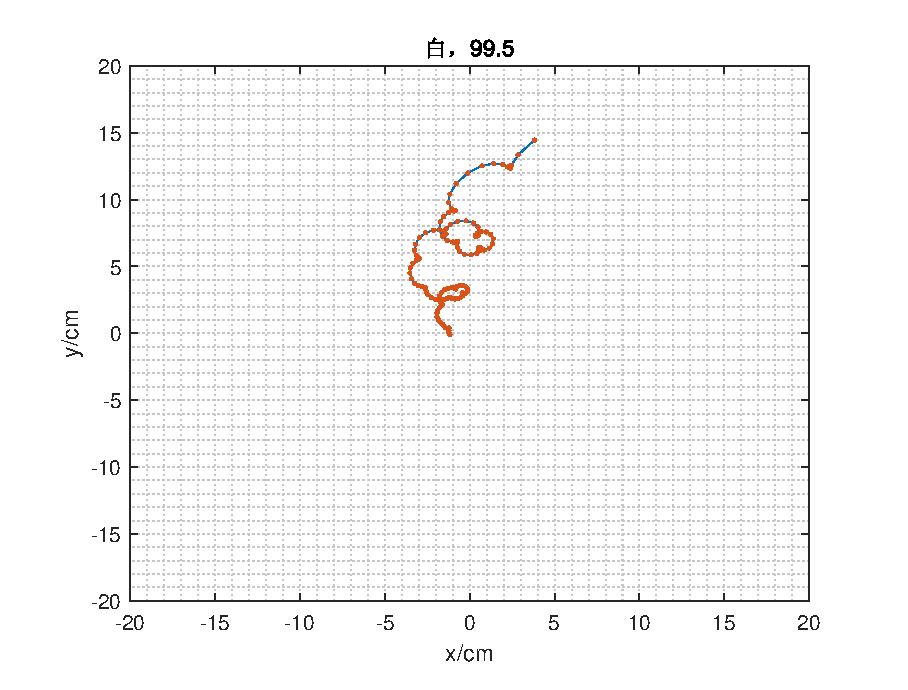
\includegraphics[width=0.48\linewidth]{./figures/w100.eps}}
		%\quad
		\subfigure[$q$=0.079]{
			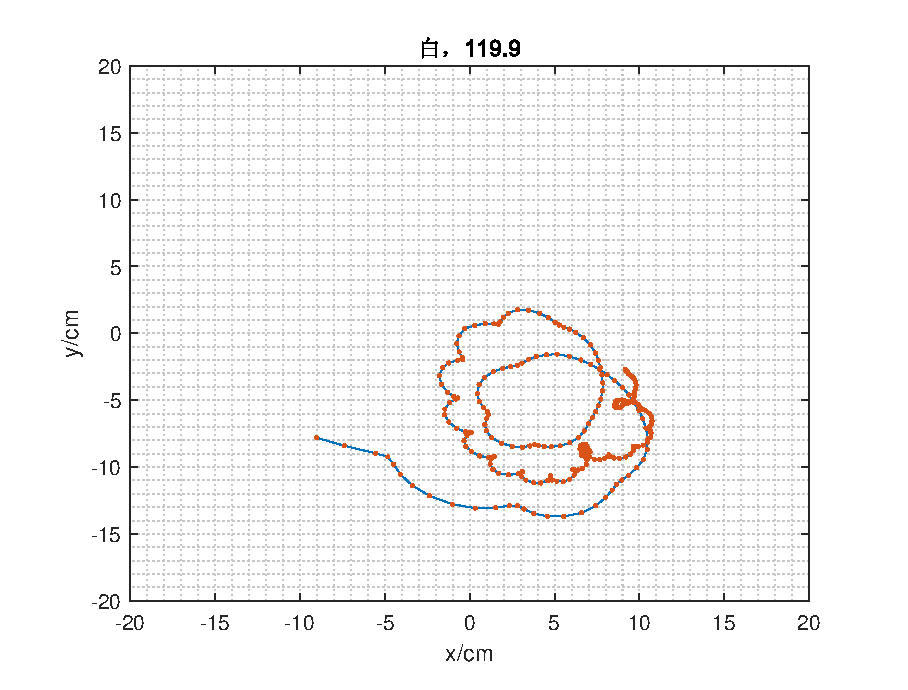
\includegraphics[width=0.48\linewidth]{./figures/w120.eps}}
	\end{figure}
	\addtocounter{figure}{-1} 
	\begin{figure}[H]
		\addtocounter{figure}{1} 
		\centering  %图片全局居中
		\subfigbottomskip=2pt %两行子图之间的行间距
		\subfigcapskip=-5pt %设置子图与子标题之间的距离
		\subfigure[$q$=0.058]{
			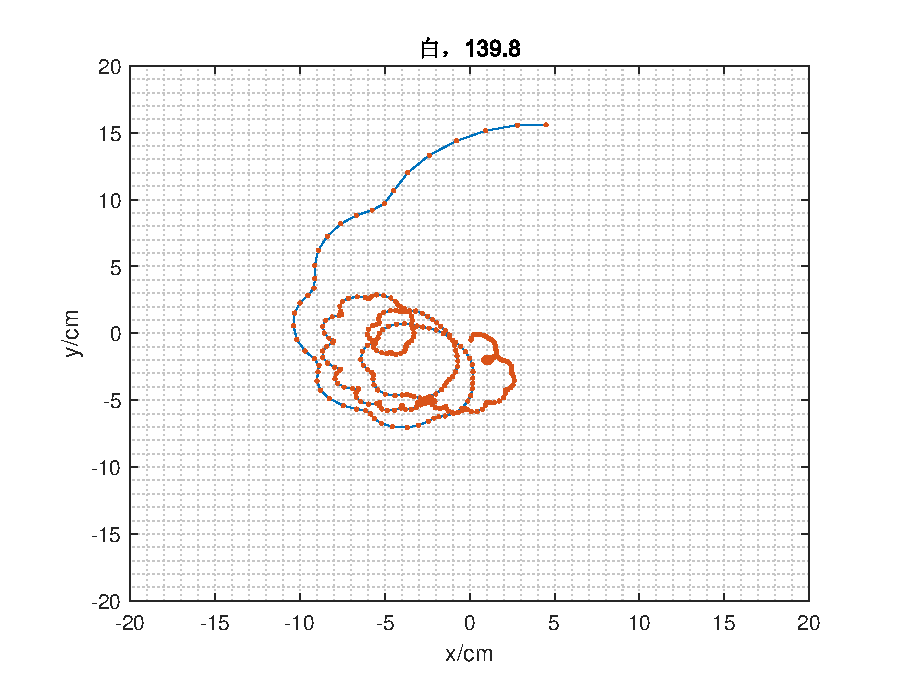
\includegraphics[width=0.48\linewidth]{./figures/w140.eps}}
		%\quad
		\subfigure[$q$=0.045]{
			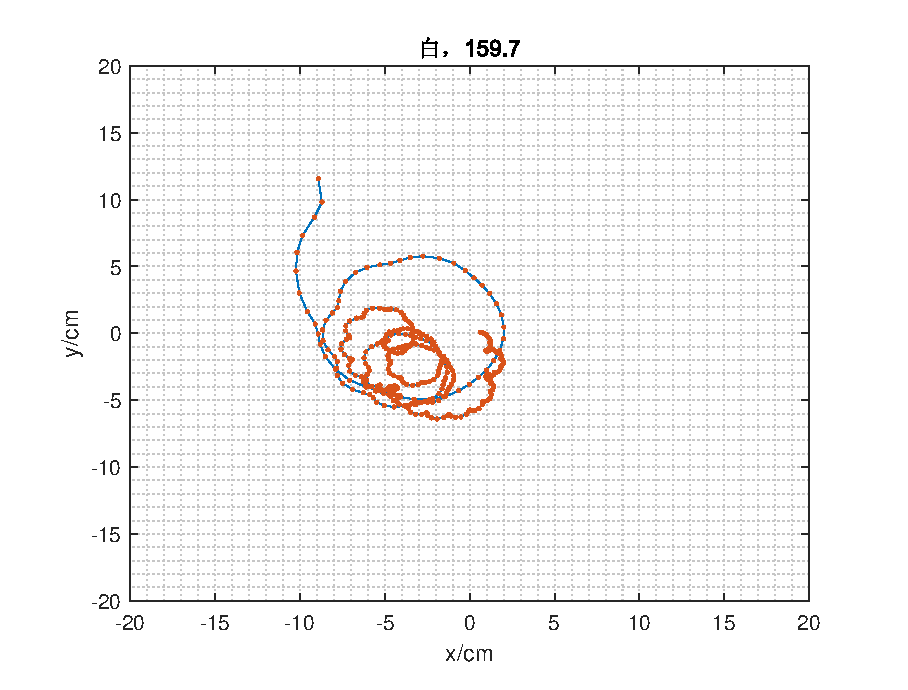
\includegraphics[width=0.48\linewidth]{./figures/w160.eps}}
	\end{figure}
	\addtocounter{figure}{-1} 
	\begin{figure}[H]
		\addtocounter{figure}{1} 
		\centering  %图片全局居中
		\subfigbottomskip=2pt %两行子图之间的行间距
		\subfigcapskip=-5pt %设置子图与子标题之间的距离
		\subfigure[$q$=0.035]{
			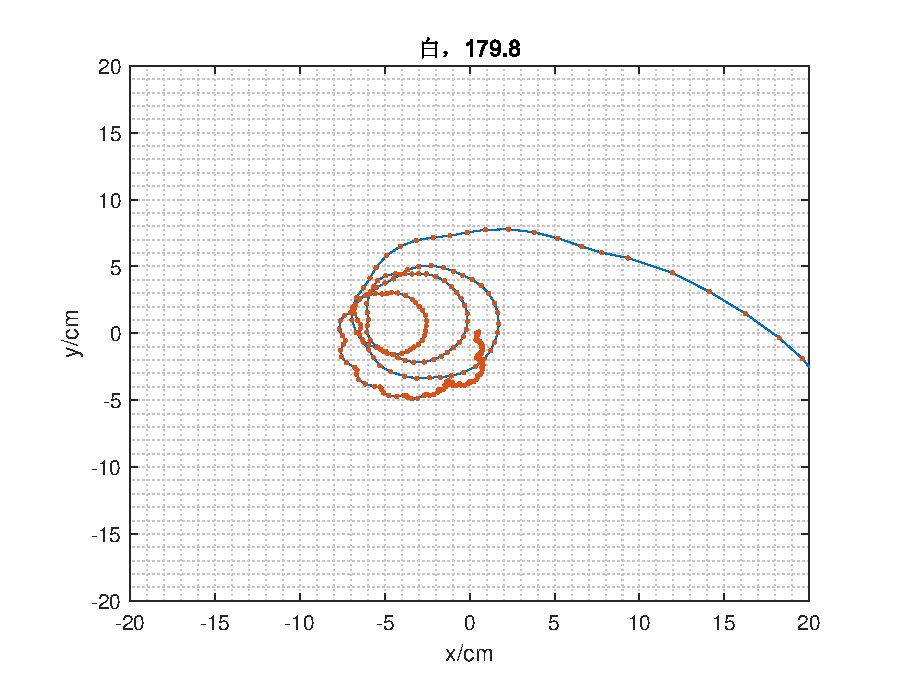
\includegraphics[width=0.48\linewidth]{./figures/w180.eps}}
		%\quad
		\subfigure[$q$=0.029]{
			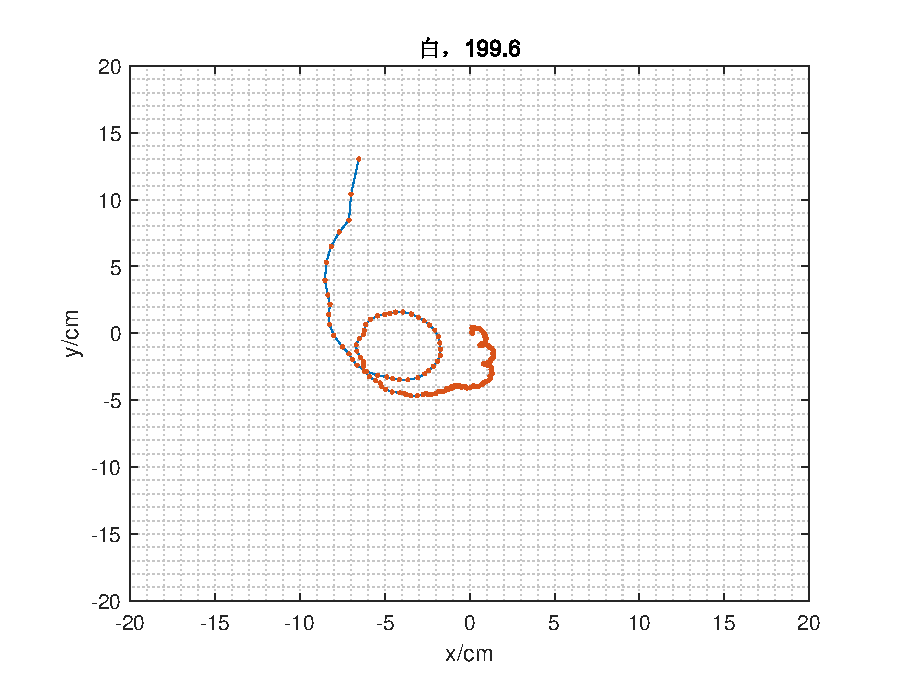
\includegraphics[width=0.48\linewidth]{./figures/w200.eps}}
		\caption{塑料小球的运动图像}
	\end{figure}
	
	\subsubsection{铝制小球}
	\begin{figure}[H]
		\centering  %图片全局居中
		\subfigbottomskip=2pt %两行子图之间的行间距
		\subfigcapskip=-5pt %设置子图与子标题之间的距离
		\subfigure[$q$=0.318]{
			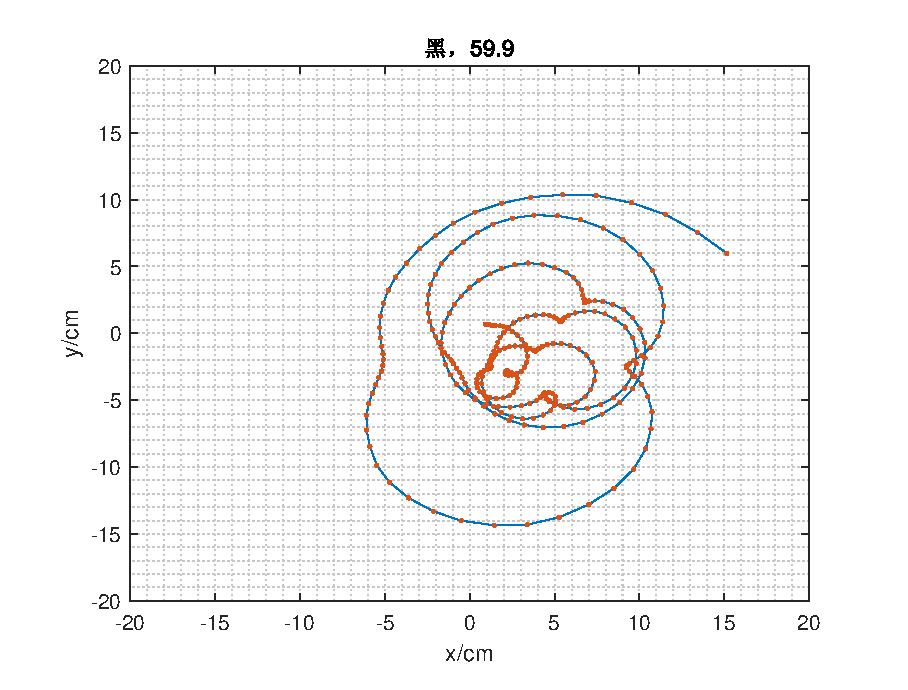
\includegraphics[width=0.48\linewidth]{./figures/b60.eps}}
		\subfigure[$q$=0.179]{
			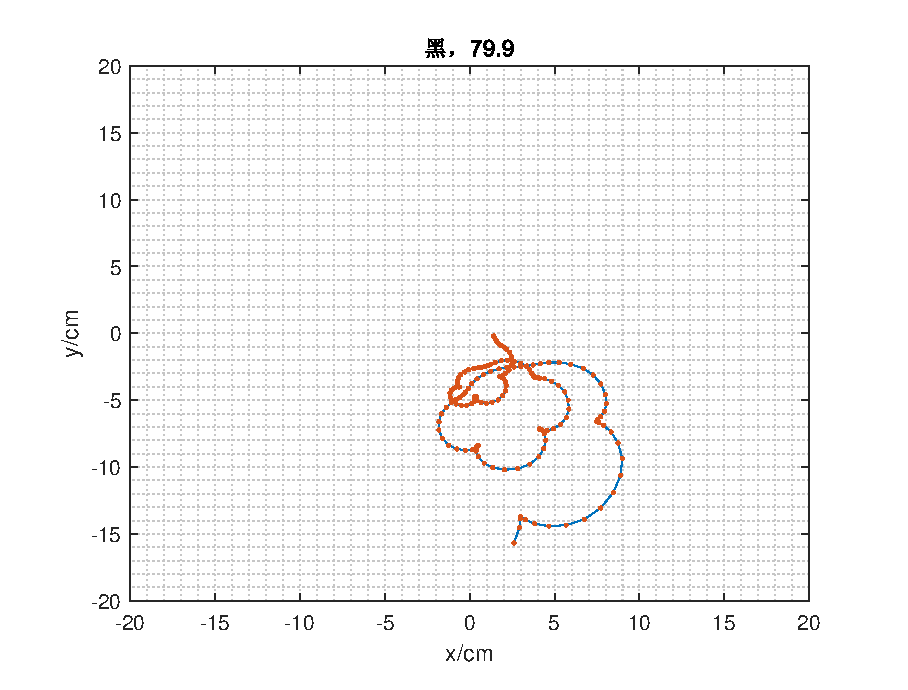
\includegraphics[width=0.48\linewidth]{./figures/b80.eps}}
	\end{figure}
	\addtocounter{figure}{-1} 
		\begin{figure}[H]
		\addtocounter{figure}{1} 
		\centering  %图片全局居中
		\subfigbottomskip=2pt %两行子图之间的行间距
		\subfigcapskip=-5pt %设置子图与子标题之间的距离
		\subfigure[$q$=0.114]{
			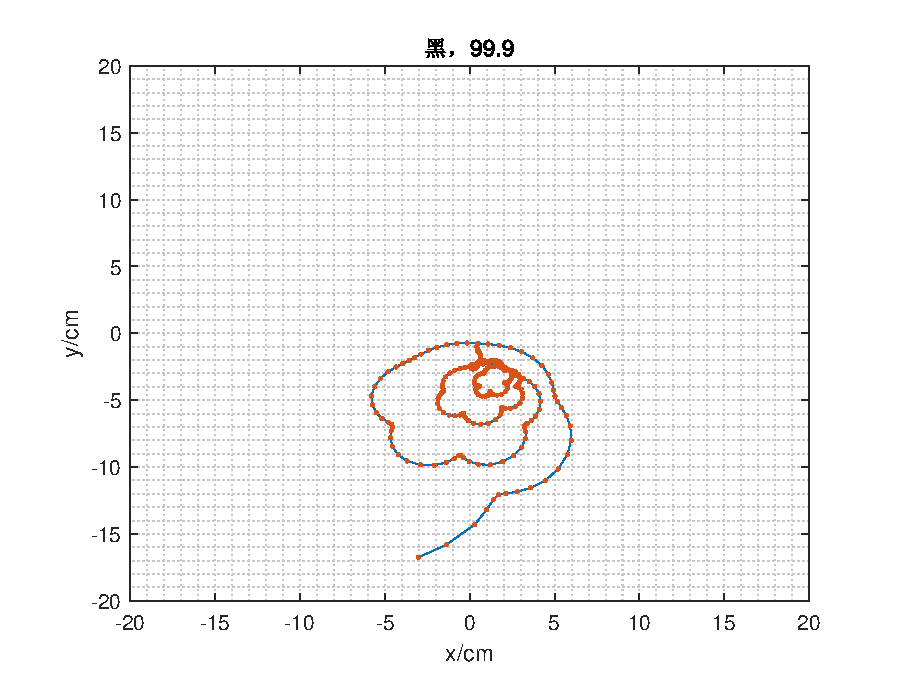
\includegraphics[width=0.48\linewidth]{./figures/b100.eps}}
		%\quad
		\subfigure[$q$=0.079]{
			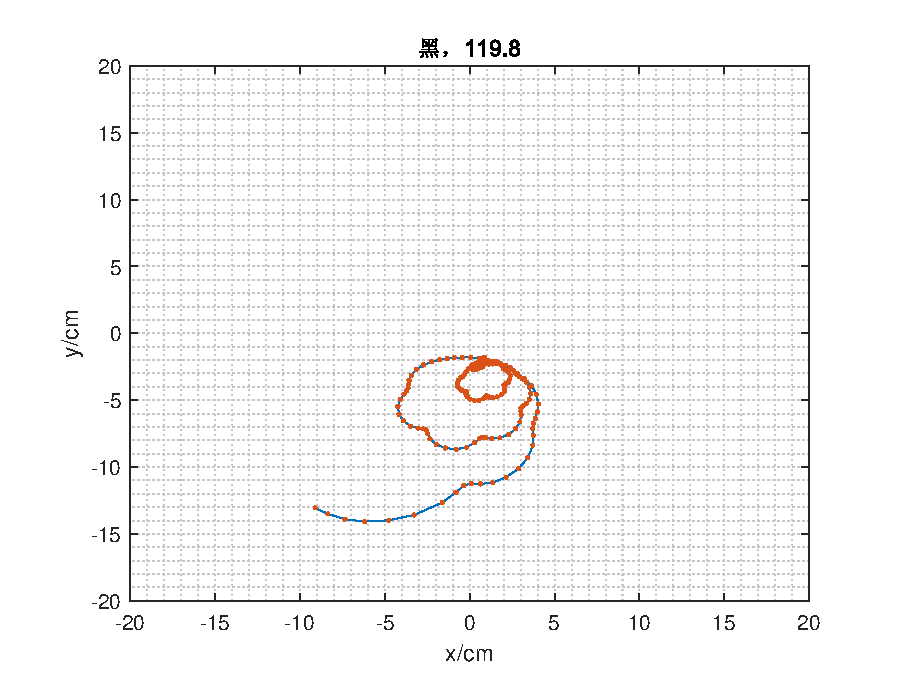
\includegraphics[width=0.48\linewidth]{./figures/b120.eps}}
		\end{figure}
		\addtocounter{figure}{-1} 
		\begin{figure}[H]
		\addtocounter{figure}{1} 
		\centering  %图片全局居中
		\subfigbottomskip=2pt %两行子图之间的行间距
		\subfigcapskip=-5pt %设置子图与子标题之间的距离
		\subfigure[$q$=0.058]{
			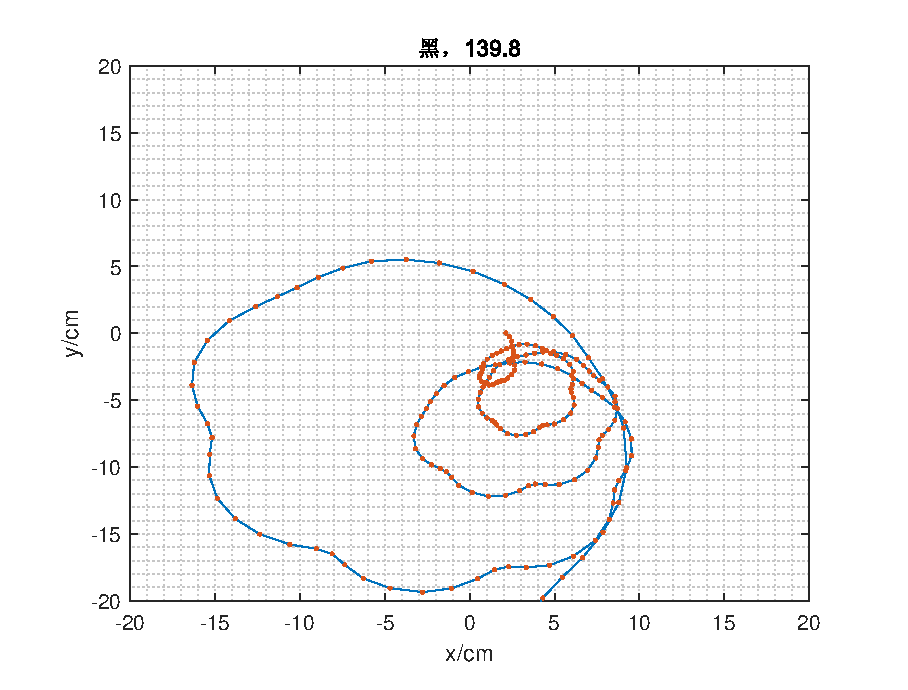
\includegraphics[width=0.48\linewidth]{./figures/b140.eps}}
		%\quad
		\subfigure[$q$=0.045]{
			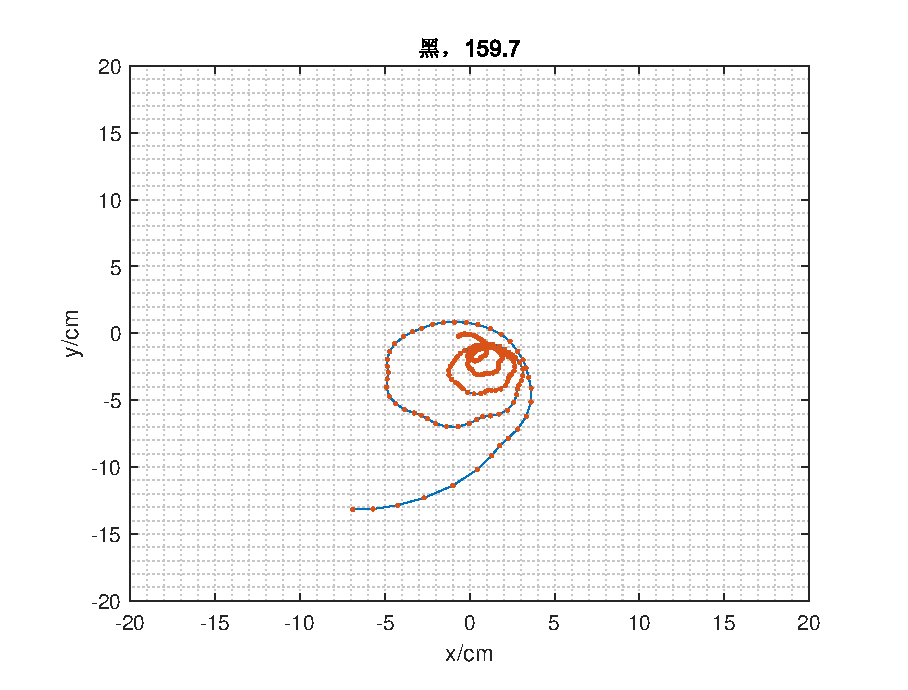
\includegraphics[width=0.48\linewidth]{./figures/b160.eps}}
		\end{figure}
		\addtocounter{figure}{-1} 
		\begin{figure}[H]
		\addtocounter{figure}{1} 
		\centering  %图片全局居中
		\subfigbottomskip=2pt %两行子图之间的行间距
		\subfigcapskip=-5pt %设置子图与子标题之间的距离
		\subfigure[$q$=0.035]{
			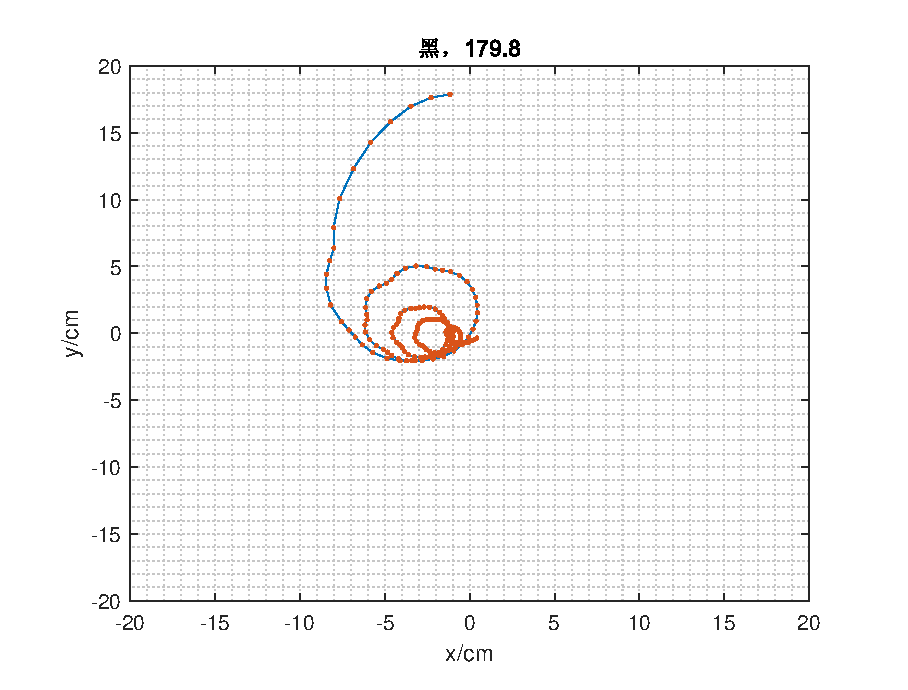
\includegraphics[width=0.48\linewidth]{./figures/b180.eps}}
		%\quad
		\subfigure[$q$=0.029]{
			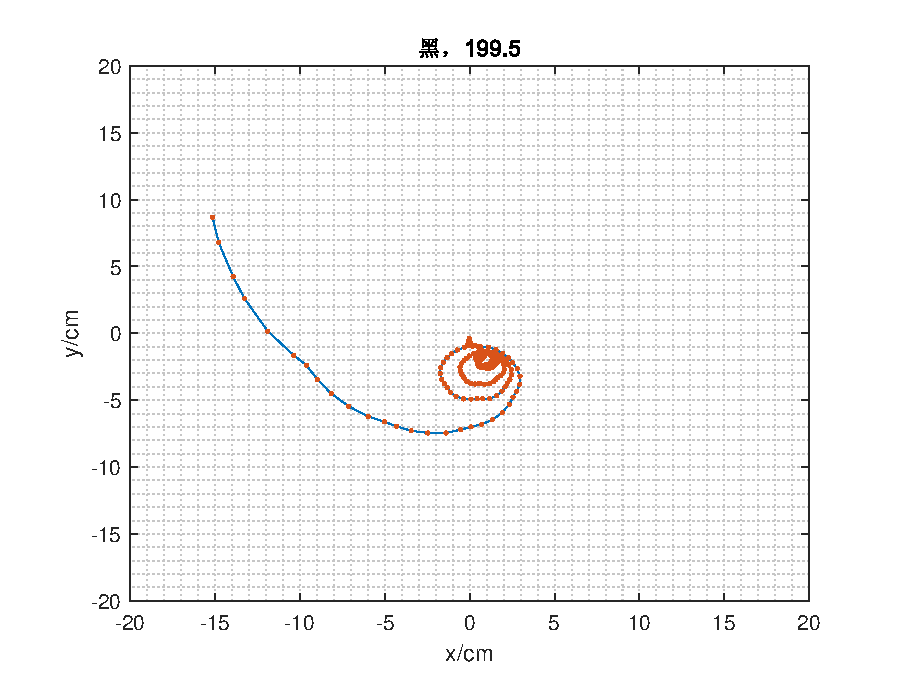
\includegraphics[width=0.48\linewidth]{./figures/b200.eps}}
		\caption{铝制小球的运动图像}
	\end{figure}
	
	\subsubsection{乒乓球}
		\begin{figure}[H]
		\centering  %图片全局居中
		\subfigbottomskip=2pt %两行子图之间的行间距
		\subfigcapskip=-5pt %设置子图与子标题之间的距离
		\subfigure[$q$=0.318]{
			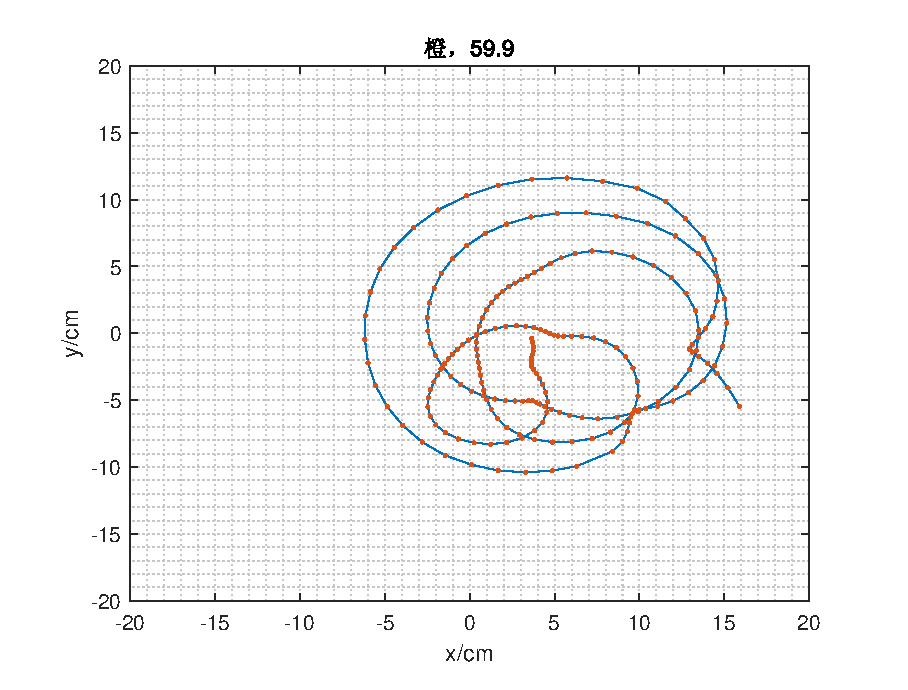
\includegraphics[width=0.48\linewidth]{./figures/o60.eps}}
		\subfigure[$q$=0.179]{
			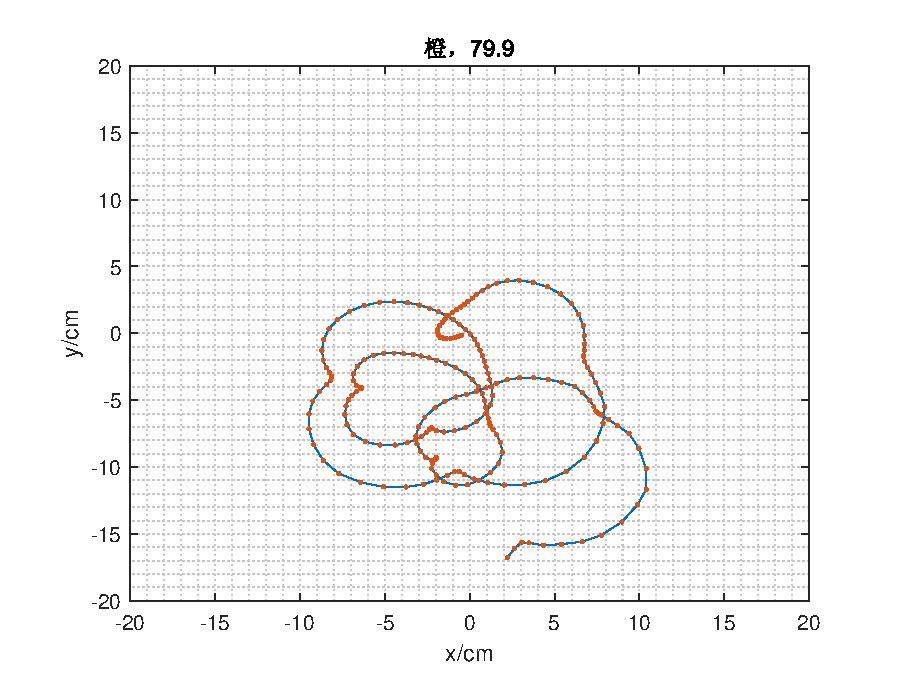
\includegraphics[width=0.48\linewidth]{./figures/o80.eps}}
		\end{figure}
		\addtocounter{figure}{-1} 
		\begin{figure}[H]
		\addtocounter{figure}{1} 
		\centering  %图片全局居中
		\subfigbottomskip=2pt %两行子图之间的行间距
		\subfigcapskip=-5pt %设置子图与子标题之间的距离
		\subfigure[$q$=0.114]{
			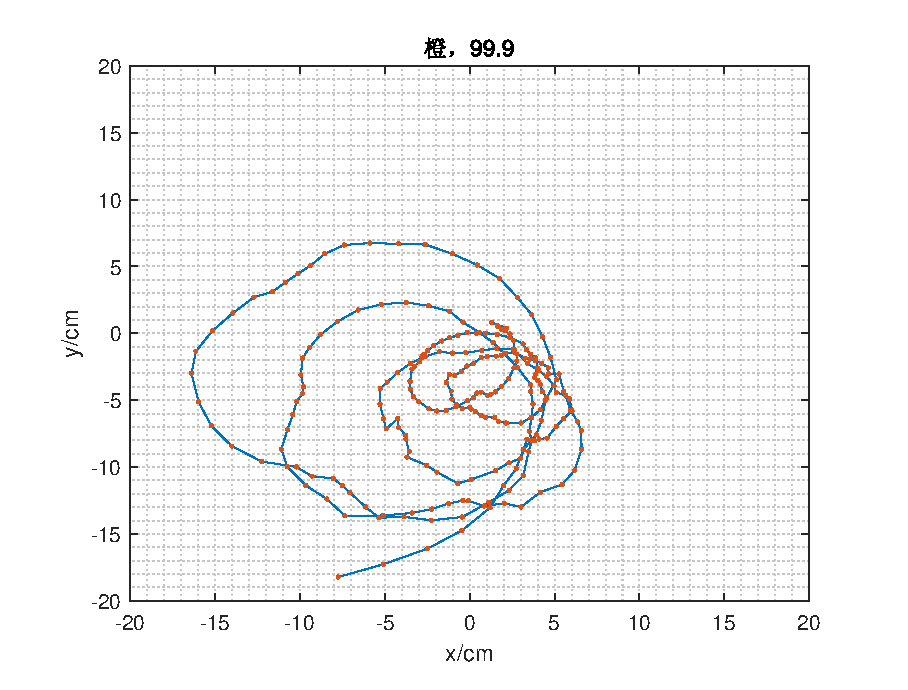
\includegraphics[width=0.48\linewidth]{./figures/o100.eps}}
		%\quad
		\subfigure[$q$=0.079]{
			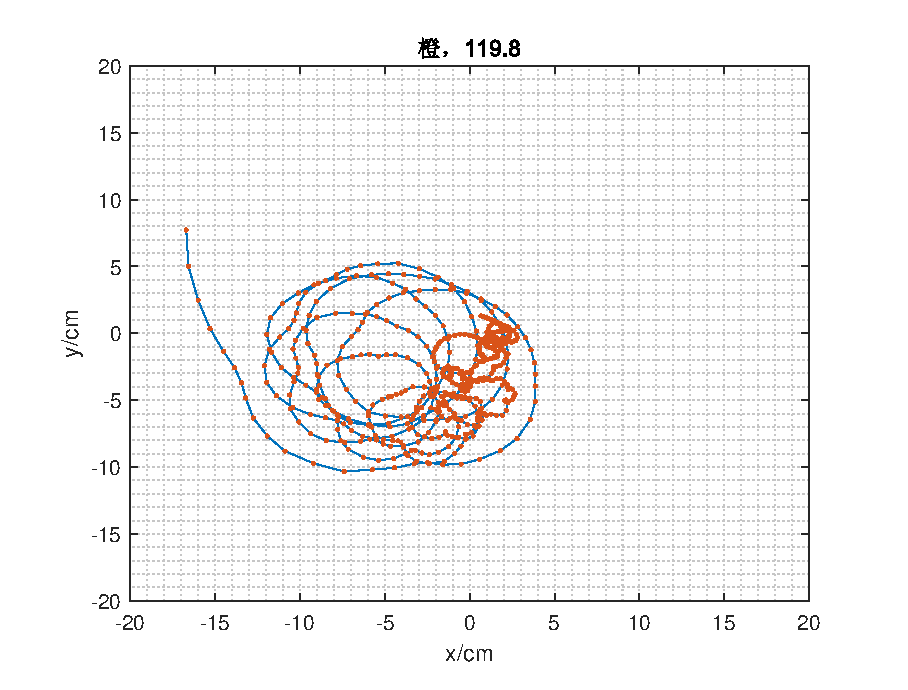
\includegraphics[width=0.48\linewidth]{./figures/o120.eps}}
		\end{figure}
		\addtocounter{figure}{-1} 
		\begin{figure}[H]
		\addtocounter{figure}{1} 
		\centering  %图片全局居中
		\subfigbottomskip=2pt %两行子图之间的行间距
		\subfigcapskip=-5pt %设置子图与子标题之间的距离
		\subfigure[$q$=0.058]{
			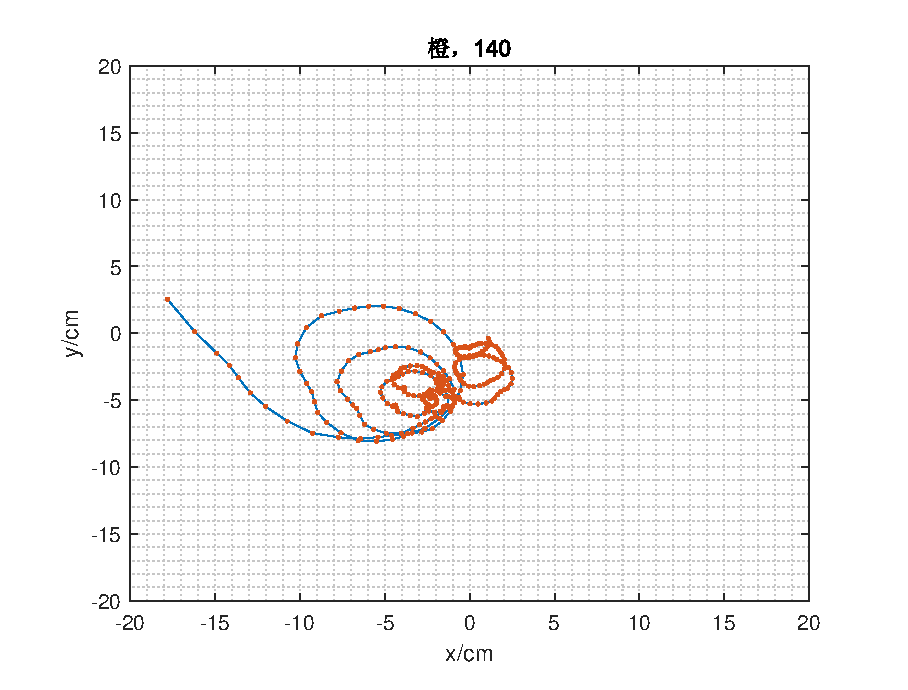
\includegraphics[width=0.48\linewidth]{./figures/o140.eps}}
		%\quad
		\subfigure[$q$=0.045]{
			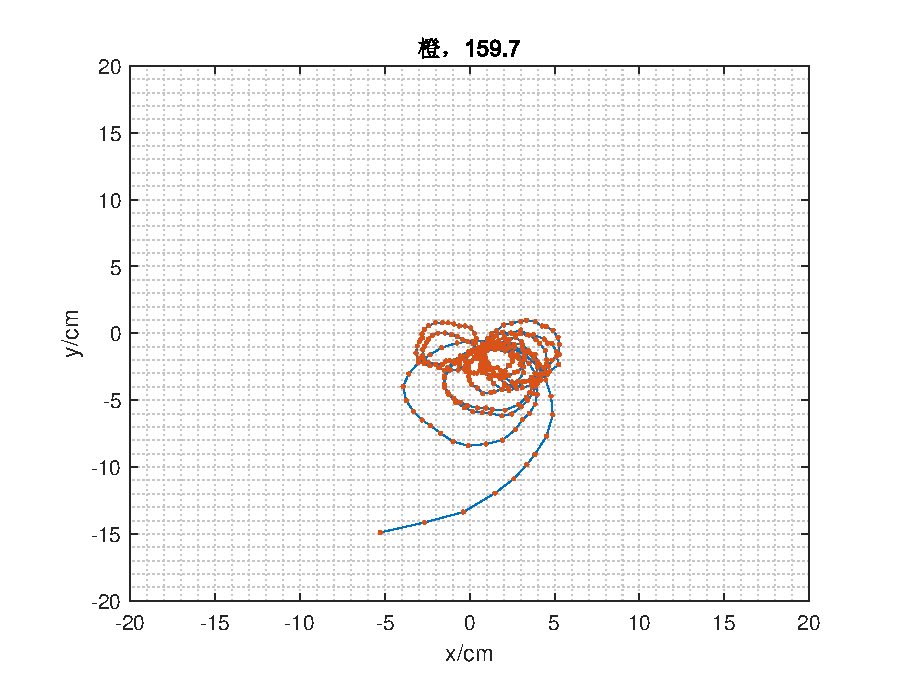
\includegraphics[width=0.48\linewidth]{./figures/o160.eps}}
		\end{figure}
		\addtocounter{figure}{-1} 
		\begin{figure}[H]
		\addtocounter{figure}{1} 
		\centering  %图片全局居中
		\subfigbottomskip=2pt %两行子图之间的行间距
		\subfigcapskip=-5pt %设置子图与子标题之间的距离
		\subfigure[$q$=0.035]{
			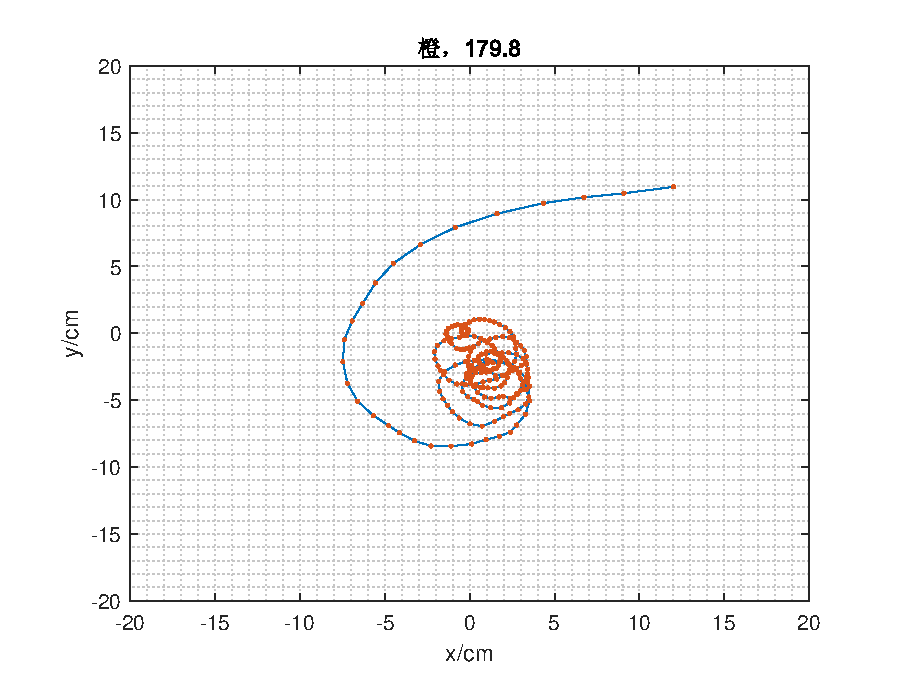
\includegraphics[width=0.48\linewidth]{./figures/o180.eps}}
		%\quad
		\subfigure[$q$=0.029]{
			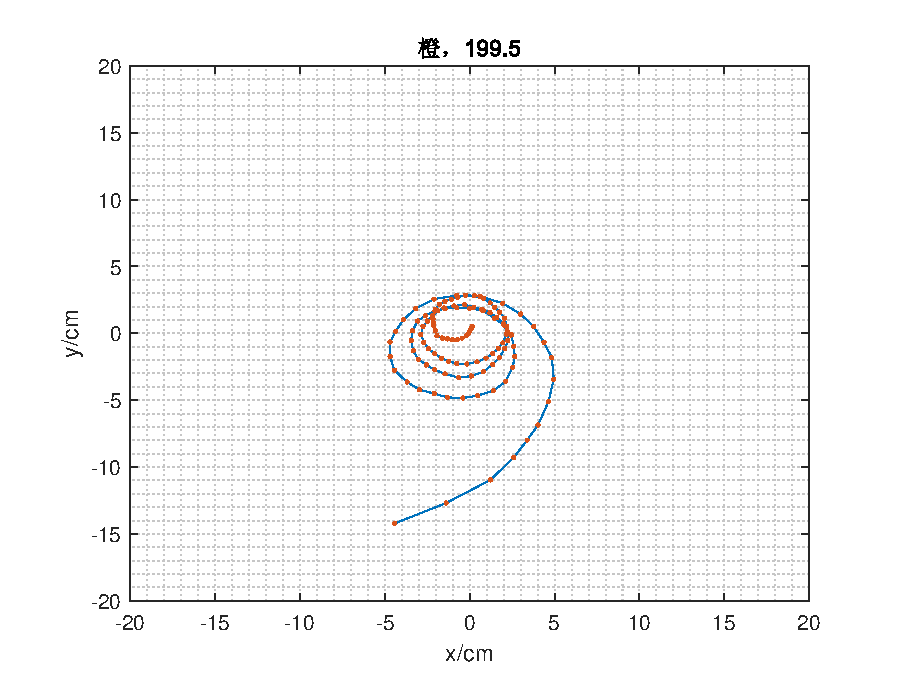
\includegraphics[width=0.48\linewidth]{./figures/o200.eps}}
		\caption{乒乓球的运动图像}
		\end{figure}
	
	\subsection{实验数据分析}
	在$q<0.5$时,小球在马鞍面上几乎不停留,以对数螺线的方式迅速滑落。但随着$q$的增大,小球在马鞍面上停留的时间变长,而且对应所绕圈数也增加,有被囚禁的迹象,但是这都只是在运动前期的现象。从图中不难发现,在运动前期小球的运动轨迹与理论分析比较类似,但是在后期呈现出对数螺线的轨迹,并快速飞出马鞍面,并没有一直被囚禁。这其实说明了我们对模型的简化欠佳,在运动后期摩擦力起到不可忽视的作用。
	
	另外我们还发现三种小球的运动轨迹差别较大,但是从运动方程上看应该一致,这是因为我们将小球都看成质点,忽略了转动,但是实验上发现小球的转动效应也比较关键。铝制小球的转动惯量比较大,看成质点是不错的近似,这从实验图像上也能看出来。
	
	\section{进一步分析}
	既然粒子失稳是因为摩擦力的影响,那我们可以在体系中加入摩擦力\upcite{main}:
	\begin{equation}
		F=-\mu \Omega\left[\frac{d}{d\tau}z(\tau)-iz(\tau)\right]
	\end{equation}
	加入摩擦力后解得运动轨迹为:
	\begin{equation}
		\begin{aligned}
			f(\tau)=&A\mathrm{e}^{(+\beta_++\epsilon)\tau}+B\mathrm{e}^{(-\beta_++\epsilon)\tau}\\&+C\mathrm{e}^{(+\beta_-+\epsilon)\tau}+D\mathrm{e}^{(-\beta_-+\epsilon)\tau}
		\end{aligned}
	\end{equation}
	其中
	\begin{equation}
		\epsilon=\frac{1}{2q}(1-q)\mu
	\end{equation}
	其永远为实数,所以足够长的时间后总会引起解的指数发散。这也是实验上永远不可能让粒子一直处于囚禁状态的原因。
	
	利用Mathematica对含摩擦项的运动方程进行求解,得到下面的运动图像:
	\begin{figure}[H]
		\centering  %图片全局居中
		\subfigbottomskip=2pt %两行子图之间的行间距
		\subfigcapskip=-5pt %设置子图与子标题之间的距离
		\subfigure[$q=0.1,\mu\Omega=0.005$时的运动轨迹]{
			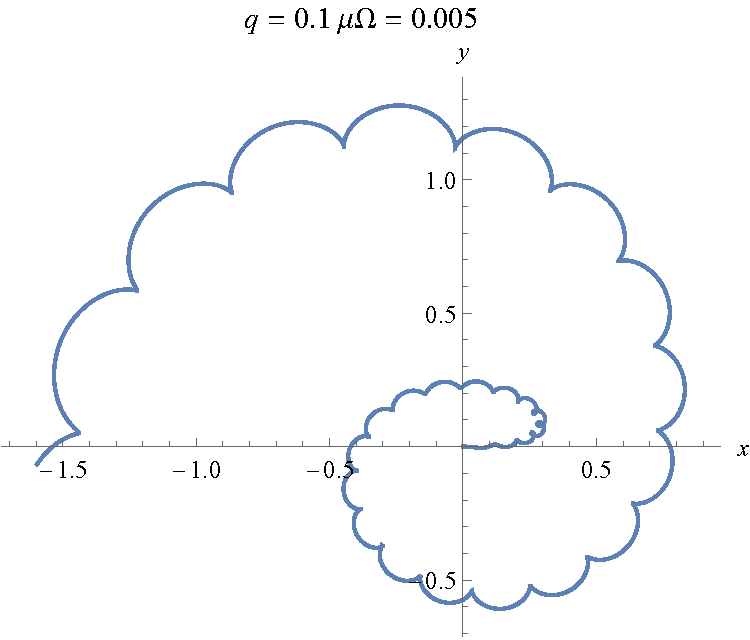
\includegraphics[width=0.48\linewidth]{figures/mu0.1.pdf}}
		\subfigure[$q=0.35,\mu\Omega=0.005$时的运动轨迹]{
			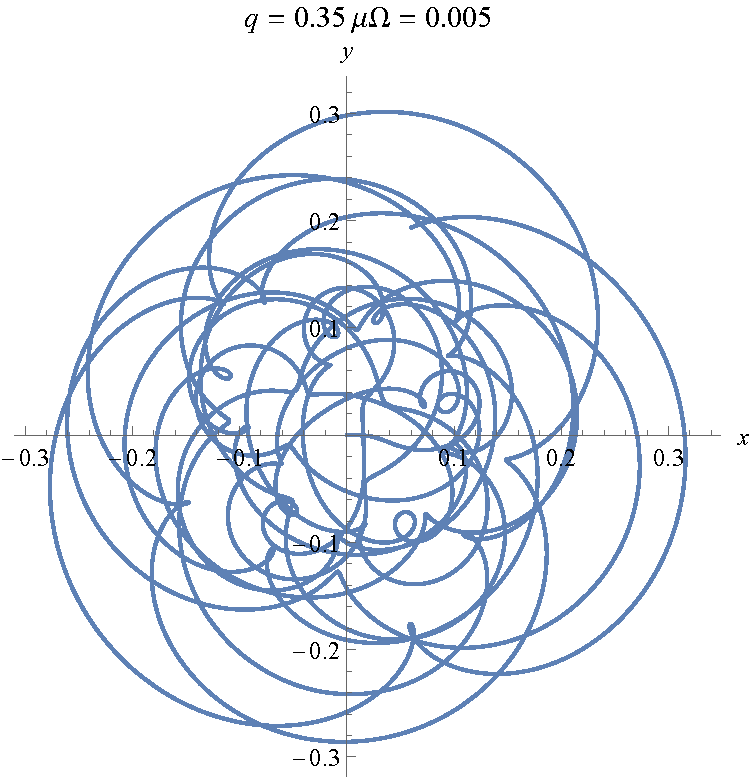
\includegraphics[width=0.48\linewidth]{figures/mu0.35.pdf}}
		\caption{转速为$40\operatorname{r/min}$时的运动轨迹}
	\end{figure}
	
	
	可以发现加入摩擦项后粒子轨迹都会有指数发散的趋势,而且将上面的理论结果与前一小节得到的实验结果相比较会发现理论与实验曲线有比较强的相似性:在运动初期运动由于摩擦的存在不是太规则,后期摩擦使得运动轨迹指数发散。
	
	另外,从实验还观测到角速度越大粒子越快进入对数螺线阶段脱离马鞍面。从方程(12)上看可以解释为$\mu\Omega$变大导致摩擦项增大。从物理上也可以直观解释为在角速度不大时,小球自转跟得上马鞍面旋转,主要受静摩擦力,摩擦力对运动贡献并不大;但是在角速度较大时,小球自转跟不上马鞍面旋转,主要受滑动摩擦力,摩擦力占主导地位。
	\section{结\quad 论}
	本次实验通过Paul机械势阱研究了质点在旋转马鞍面上的运动状态,发现$q<0.5$时,在运动初期,质点的运动与无摩擦情况下类似,被囚禁在一块区域内,但是由于摩擦力的存在,以及小球不能完全简化为质点模型,在运动后期小球会以对数螺线的方式快速飞出马鞍面;在$q>0.5$时,小球则是在一开始便快速飞出马鞍面。
	
	查阅文献\upcite{QIT1}\upcite{QIT2}得知,四极离子阱的电势分布为
	\begin{equation}
		\Phi(x,y,t)=\left[U+V\cos(\omega_{rf}f)\right]\frac{x^2-y^2}{2{r_0}^2}
	\end{equation}
	不难发现与机械阱一样具有马鞍面的形式,所以我们可以使用机械阱大致模拟四极离子阱囚禁离子的工作原理。
	
	%\bibliography{article}】
	\small
	\bibliographystyle{gbt7714-numerical}
	\bibliography{article}
\end{multicols}

\end{document}
